% GNUPLOT: LaTeX picture with Postscript
\begingroup
  \makeatletter
  \providecommand\color[2][]{%
    \GenericError{(gnuplot) \space\space\space\@spaces}{%
      Package color not loaded in conjunction with
      terminal option `colourtext'%
    }{See the gnuplot documentation for explanation.%
    }{Either use 'blacktext' in gnuplot or load the package
      color.sty in LaTeX.}%
    \renewcommand\color[2][]{}%
  }%
  \providecommand\includegraphics[2][]{%
    \GenericError{(gnuplot) \space\space\space\@spaces}{%
      Package graphicx or graphics not loaded%
    }{See the gnuplot documentation for explanation.%
    }{The gnuplot epslatex terminal needs graphicx.sty or graphics.sty.}%
    \renewcommand\includegraphics[2][]{}%
  }%
  \providecommand\rotatebox[2]{#2}%
  \@ifundefined{ifGPcolor}{%
    \newif\ifGPcolor
    \GPcolortrue
  }{}%
  \@ifundefined{ifGPblacktext}{%
    \newif\ifGPblacktext
    \GPblacktexttrue
  }{}%
  % define a \g@addto@macro without @ in the name:
  \let\gplgaddtomacro\g@addto@macro
  % define empty templates for all commands taking text:
  \gdef\gplbacktext{}%
  \gdef\gplfronttext{}%
  \makeatother
  \ifGPblacktext
    % no textcolor at all
    \def\colorrgb#1{}%
    \def\colorgray#1{}%
  \else
    % gray or color?
    \ifGPcolor
      \def\colorrgb#1{\color[rgb]{#1}}%
      \def\colorgray#1{\color[gray]{#1}}%
      \expandafter\def\csname LTw\endcsname{\color{white}}%
      \expandafter\def\csname LTb\endcsname{\color{black}}%
      \expandafter\def\csname LTa\endcsname{\color{black}}%
      \expandafter\def\csname LT0\endcsname{\color[rgb]{1,0,0}}%
      \expandafter\def\csname LT1\endcsname{\color[rgb]{0,1,0}}%
      \expandafter\def\csname LT2\endcsname{\color[rgb]{0,0,1}}%
      \expandafter\def\csname LT3\endcsname{\color[rgb]{1,0,1}}%
      \expandafter\def\csname LT4\endcsname{\color[rgb]{0,1,1}}%
      \expandafter\def\csname LT5\endcsname{\color[rgb]{1,1,0}}%
      \expandafter\def\csname LT6\endcsname{\color[rgb]{0,0,0}}%
      \expandafter\def\csname LT7\endcsname{\color[rgb]{1,0.3,0}}%
      \expandafter\def\csname LT8\endcsname{\color[rgb]{0.5,0.5,0.5}}%
    \else
      % gray
      \def\colorrgb#1{\color{black}}%
      \def\colorgray#1{\color[gray]{#1}}%
      \expandafter\def\csname LTw\endcsname{\color{white}}%
      \expandafter\def\csname LTb\endcsname{\color{black}}%
      \expandafter\def\csname LTa\endcsname{\color{black}}%
      \expandafter\def\csname LT0\endcsname{\color{black}}%
      \expandafter\def\csname LT1\endcsname{\color{black}}%
      \expandafter\def\csname LT2\endcsname{\color{black}}%
      \expandafter\def\csname LT3\endcsname{\color{black}}%
      \expandafter\def\csname LT4\endcsname{\color{black}}%
      \expandafter\def\csname LT5\endcsname{\color{black}}%
      \expandafter\def\csname LT6\endcsname{\color{black}}%
      \expandafter\def\csname LT7\endcsname{\color{black}}%
      \expandafter\def\csname LT8\endcsname{\color{black}}%
    \fi
  \fi
    \setlength{\unitlength}{0.0500bp}%
    \ifx\gptboxheight\undefined%
      \newlength{\gptboxheight}%
      \newlength{\gptboxwidth}%
      \newsavebox{\gptboxtext}%
    \fi%
    \setlength{\fboxrule}{0.5pt}%
    \setlength{\fboxsep}{1pt}%
\begin{picture}(7200.00,5040.00)%
    \gplgaddtomacro\gplbacktext{%
      \csname LTb\endcsname%%
      \put(990,709){\makebox(0,0)[r]{\strut{}$10000$}}%
      \put(990,2594){\makebox(0,0)[r]{\strut{}$100000$}}%
      \put(990,4479){\makebox(0,0)[r]{\strut{}$1\times10^{6}$}}%
      \put(1690,220){\makebox(0,0){\strut{}$10$}}%
      \put(2826,220){\makebox(0,0){\strut{}$20$}}%
      \put(3963,220){\makebox(0,0){\strut{}$30$}}%
      \put(5099,220){\makebox(0,0){\strut{}$40$}}%
      \put(6235,220){\makebox(0,0){\strut{}$50$}}%
      \colorrgb{0.00,0.62,0.45}%%
      \put(1690,1094){\rotatebox{33}{\makebox(0,0)[l]{\strut{}k = 0.096}}}%
      \colorrgb{0.34,0.71,0.91}%%
      \put(2826,2027){\rotatebox{29}{\makebox(0,0)[l]{\strut{}k = 0.0754}}}%
      \colorrgb{0.00,0.62,0.45}%%
      \put(1690,1094){\rotatebox{33}{\makebox(0,0)[l]{\strut{}k = 0.096}}}%
      \colorrgb{0.34,0.71,0.91}%%
      \put(2826,2027){\rotatebox{29}{\makebox(0,0)[l]{\strut{}k = 0.0754}}}%
      \colorrgb{0.00,0.62,0.45}%%
      \put(1690,1094){\rotatebox{33}{\makebox(0,0)[l]{\strut{}k = 0.096}}}%
      \colorrgb{0.34,0.71,0.91}%%
      \put(2826,2027){\rotatebox{29}{\makebox(0,0)[l]{\strut{}k = 0.0754}}}%
      \colorrgb{0.00,0.62,0.45}%%
      \put(1690,1094){\rotatebox{33}{\makebox(0,0)[l]{\strut{}k = 0.096}}}%
      \colorrgb{0.34,0.71,0.91}%%
      \put(2826,2027){\rotatebox{29}{\makebox(0,0)[l]{\strut{}k = 0.0754}}}%
      \colorrgb{0.12,0.52,0.11}%%
      \put(1690,1094){\rotatebox{33}{\makebox(0,0)[l]{\strut{}k = 0.096}}}%
      \colorrgb{0.24,0.25,0.84}%%
      \put(2826,2027){\rotatebox{29}{\makebox(0,0)[l]{\strut{}k = 0.0754}}}%
      \colorrgb{0.12,0.52,0.11}%%
      \put(1690,1094){\rotatebox{33}{\makebox(0,0)[l]{\strut{}k = 0.096}}}%
      \colorrgb{0.24,0.25,0.84}%%
      \put(2826,2027){\rotatebox{29}{\makebox(0,0)[l]{\strut{}k = 0.0754}}}%
      \colorrgb{0.12,0.52,0.11}%%
      \put(1690,1094){\rotatebox{33}{\makebox(0,0)[l]{\strut{}k = 0.096}}}%
      \colorrgb{0.24,0.25,0.84}%%
      \put(2826,2027){\rotatebox{29}{\makebox(0,0)[l]{\strut{}k = 0.0754}}}%
      \colorrgb{0.12,0.52,0.11}%%
      \put(1690,1094){\rotatebox{33}{\makebox(0,0)[l]{\strut{}k = 0.096}}}%
      \colorrgb{0.24,0.25,0.84}%%
      \put(2826,2027){\rotatebox{29}{\makebox(0,0)[l]{\strut{}k = 0.0754}}}%
      \colorrgb{0.12,0.52,0.11}%%
      \put(1690,1094){\rotatebox{33}{\makebox(0,0)[l]{\strut{}k = 0.096}}}%
      \colorrgb{0.24,0.25,0.84}%%
      \put(2826,2027){\rotatebox{29}{\makebox(0,0)[l]{\strut{}k = 0.0754}}}%
      \csname LTb\endcsname%%
      \put(554,-2147483647){\makebox(0,0)[l]{\strut{}k = 0.096}}%
      \colorrgb{0.12,0.52,0.11}%%
      \put(1690,1094){\rotatebox{33}{\makebox(0,0)[l]{\strut{}k = 0.096}}}%
      \colorrgb{0.24,0.25,0.84}%%
      \put(2826,2027){\rotatebox{29}{\makebox(0,0)[l]{\strut{}k = 0.0754}}}%
      \colorrgb{0.12,0.52,0.11}%%
      \put(1690,1094){\rotatebox{33}{\makebox(0,0)[l]{\strut{}k = 0.096}}}%
      \colorrgb{0.24,0.25,0.84}%%
      \put(2826,2027){\rotatebox{29}{\makebox(0,0)[l]{\strut{}k = 0.0754}}}%
      \colorrgb{0.12,0.52,0.11}%%
      \put(1690,1094){\rotatebox{33}{\makebox(0,0)[l]{\strut{}k = 0.096}}}%
      \colorrgb{0.24,0.25,0.84}%%
      \put(2826,2027){\rotatebox{29}{\makebox(0,0)[l]{\strut{}k = 0.0754}}}%
      \colorrgb{0.12,0.52,0.11}%%
      \put(1690,1094){\rotatebox{33}{\makebox(0,0)[l]{\strut{}k = 0.096}}}%
      \colorrgb{0.24,0.25,0.84}%%
      \put(2826,2027){\rotatebox{29}{\makebox(0,0)[l]{\strut{}k = 0.0754}}}%
      \colorrgb{0.12,0.52,0.11}%%
      \put(1690,1094){\rotatebox{33}{\makebox(0,0)[l]{\strut{}k = 0.096}}}%
      \colorrgb{0.24,0.25,0.84}%%
      \put(2826,2027){\rotatebox{29}{\makebox(0,0)[l]{\strut{}k = 0.0754}}}%
      \colorrgb{0.84,0.60,0.02}%%
      \put(1690,1094){\rotatebox{33}{\makebox(0,0)[l]{\strut{}k = 0.096}}}%
      \colorrgb{0.24,0.25,0.84}%%
      \put(2826,2027){\rotatebox{29}{\makebox(0,0)[l]{\strut{}k = 0.0754}}}%
      \colorrgb{0.02,0.84,0.60}%%
      \put(1690,1094){\rotatebox{33}{\makebox(0,0)[l]{\strut{}k = 0.096}}}%
      \colorrgb{0.24,0.25,0.84}%%
      \put(2826,2027){\rotatebox{29}{\makebox(0,0)[l]{\strut{}k = 0.0754}}}%
      \colorrgb{0.12,0.52,0.11}%%
      \put(1690,1094){\rotatebox{33}{\makebox(0,0)[l]{\strut{}k = 0.096}}}%
      \colorrgb{0.24,0.25,0.84}%%
      \put(2826,2027){\rotatebox{29}{\makebox(0,0)[l]{\strut{}k = 0.0754}}}%
      \colorrgb{0.12,0.52,0.11}%%
      \put(1690,1094){\rotatebox{33}{\makebox(0,0)[l]{\strut{}k = 0.096}}}%
      \colorrgb{0.24,0.25,0.84}%%
      \put(2826,2027){\rotatebox{29}{\makebox(0,0)[l]{\strut{}k = 0.0754}}}%
      \colorrgb{0.12,0.52,0.11}%%
      \put(1690,1094){\rotatebox{33}{\makebox(0,0)[l]{\strut{}k = 0.096}}}%
      \colorrgb{0.24,0.25,0.84}%%
      \put(2826,2027){\rotatebox{29}{\makebox(0,0)[l]{\strut{}k = 0.0754}}}%
      \colorrgb{0.12,0.52,0.11}%%
      \put(1690,1094){\rotatebox{33}{\makebox(0,0)[l]{\strut{}k = 0.096}}}%
      \colorrgb{0.24,0.25,0.84}%%
      \put(2826,2027){\rotatebox{29}{\makebox(0,0)[l]{\strut{}k = 0.0754}}}%
      \colorrgb{0.12,0.52,0.11}%%
      \put(1690,1094){\rotatebox{33}{\makebox(0,0)[l]{\strut{}k = 0.096}}}%
      \colorrgb{0.24,0.25,0.84}%%
      \put(2826,2027){\rotatebox{29}{\makebox(0,0)[l]{\strut{}k = 0.0754}}}%
    }%
    \gplgaddtomacro\gplfronttext{%
      \csname LTb\endcsname%%
      \put(3962,4709){\makebox(0,0){\strut{}Initial exponential growth, fit with $e^{kx}$}}%
    }%
    \gplbacktext
    \put(0,0){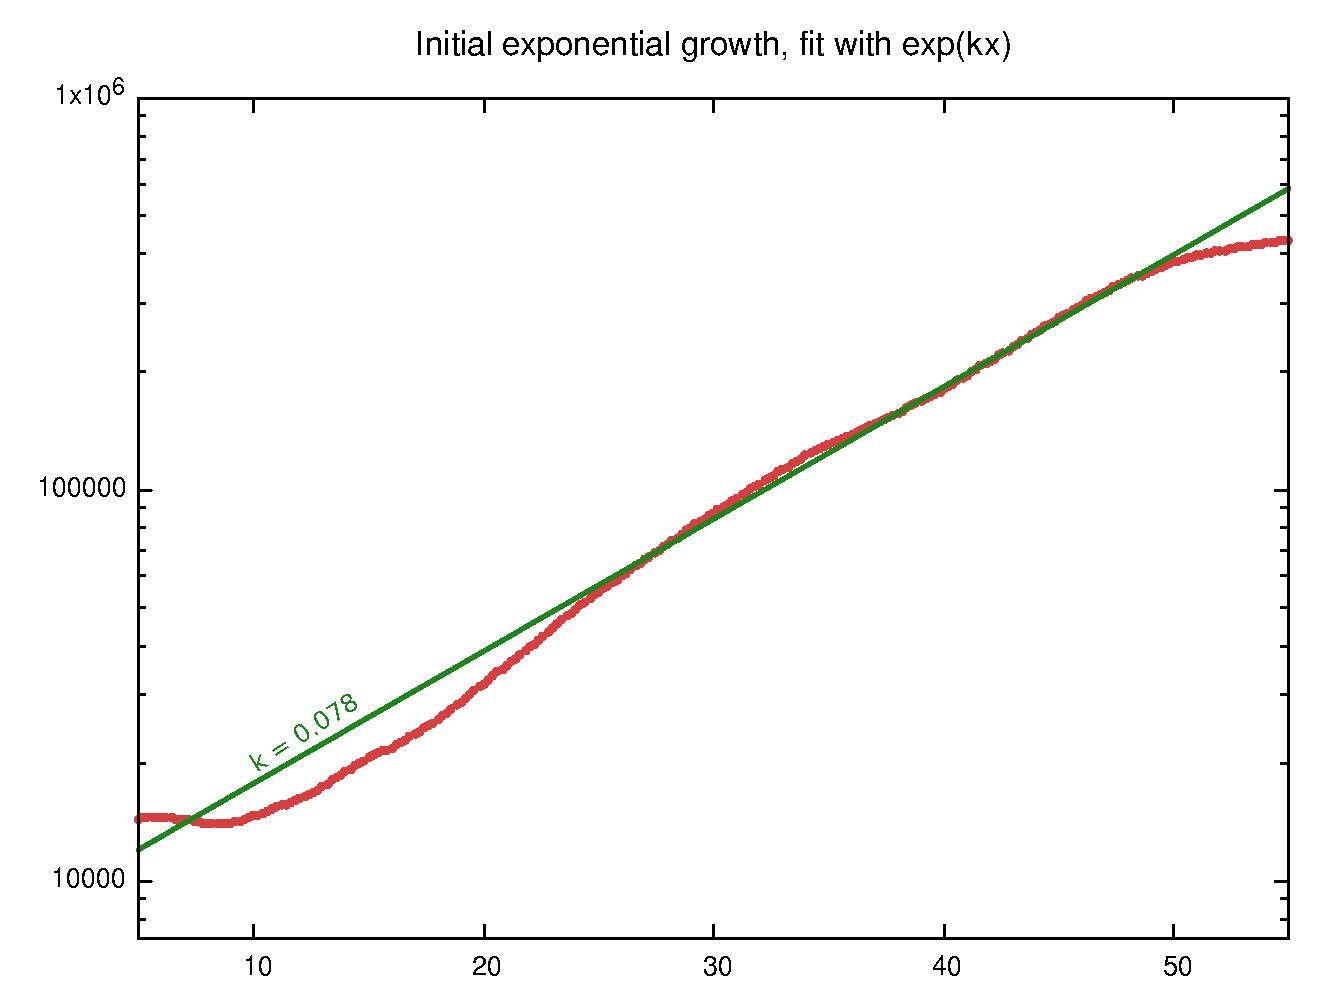
\includegraphics{/home/gab/tesi_magistrale/data/3D_model/run2/number_type1_log_zoom}}%
    \gplfronttext
  \end{picture}%
\endgroup
